\subsection{容斥问题}

\subsubsection{容斥原理}

\paragraph{容斥原理} 设 $A, B$ 是有限集合,则有:
\[
	|A \cup B| = |A| + |B| - |A \cap B|
\]

\begin{center}
	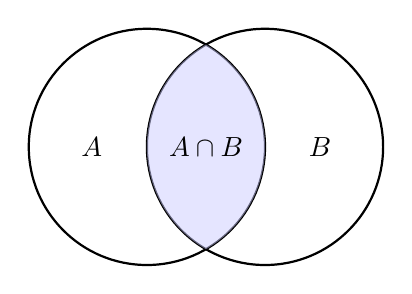
\begin{tikzpicture}
		% Draw circles
		\draw[thick] (0,0) circle (1.5);
		\draw[thick] (1.5,0) circle (1.5);
		% Labels
		\node at (-0.7,0) {$A$};
		\node at (2.2,0) {$B$};
		% Intersection shading
		\begin{scope}
			\clip (0,0) circle (1.5);
			\fill[blue!20, opacity=0.5] (1.5,0) circle (1.5);
		\end{scope}
		% Intersection label
		\node at (0.75,0) {$A \cap B$};
	\end{tikzpicture}
\end{center}

\begin{center}
	\textbf{图\thesubsubsection-\thefigure:集合 $A$ 与 $B$ 的并集与交集示意图}
\end{center}